\section{Komunikacja między klientem a serwerem}
%Specyfiką problemu jest jego dwuetapowość. W pierwszym etapipe klient inicjuje połączenie jednorazowo wysyłając zapytanie zawierające informacje o aplikacji, którą klient chce uruchomić oraz identyfikatorze klienta. W drugiej kolejności wymagane jest utworzenie kanału komunikacyjnego między klientem a procesem aplikacji. 

Do realizacji zadania komunikacji między klientem a serwerem stworzony został prosty serwer WWW działający w oparciu o protokół \emph{HTTP}. Jego architektura została przedstawiona na rysunku \ref{fig:arch-www}. Jako zasób domyślny udostępnia on listę dostępnych aplikacji, które klient może uruchomić. Inicjalizacja połączenia polega na wysłaniu przez klienta identyfikatora wybranej aplikacji. Serwer po pomyślnej weryfikacji przydziela klientowi unikatowy identyfikator sesji, uruchamia proces aplikacji i wysyła klientowi skrypt w języku \emph{JavaScript} zajmujący się przetwarzaniem po stronie przeglądarki. Każde zapytanie klienta jest weryfikowane za pomocą modułu \emph{ACL}\footnote{ang. Access Control List}, który sprawdza czy konfiguracja serwera zezwala na uruchamianie żądanych aplikacji. Szczegółowy opis modułu przedstawiono w sekcji \ref{sec:server-security}.

\begin{figure}[H]
\centering
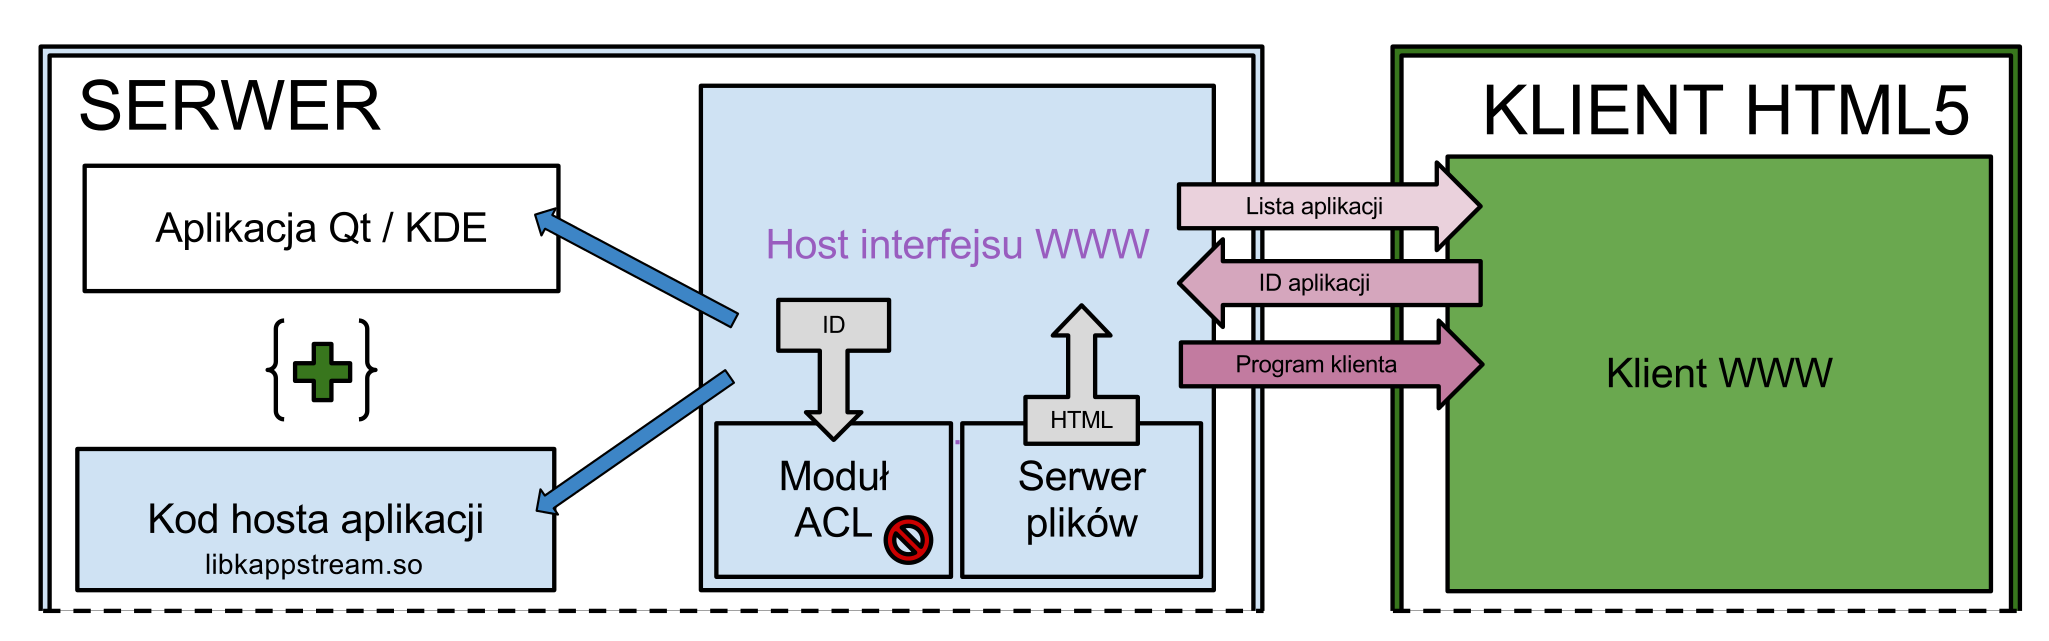
\includegraphics[width=1.0\linewidth]{img/arch-www}
\caption{Schemat komunikacji z serwerem WWW.}
\label{fig:arch-www}
\end{figure}

\section{Komunikacja między klientem a aplikacją}

Do rozwiązania tego problemu konieczne jest utworzenie ciągłego kanału komunikacyjnego między klientem a procesem aplikacji, za pomocą którego będzie możliwe przesyłanie informacji o wyglądzie interfejsu aplikacji oraz informowanie aplikacji o zdarzeniach generowanych przez użytkownika po stronie przeglądarki. Jako, że za cel przyjęte zostało założenie o nieingerowaniu bezpośrednio w kod skompilowanych już aplikacji, głównym założeniem jest skorzystanie z techniki wstrzykiwania kodu biblioteki dynamicznej do przestrzeni pamięciowej procesu aplikacji tuż przed jego uruchomieniem. Kod ten ma za zadanie utrzymanie połączenia oraz transmisję danych między klientem a aplikacją. Dokładny sposób użycia tej techniki jest przedstawiony w sekcji \ref{sec:ldpreload}. W zaprojektowanym rozwiązaniu komunikacja między aplikacją na serwerze a klientem jest bezpośrednia, z pominięciem procesu głównego serwera opisanego w poprzednim podrozdziale.

\begin{figure}[H]
\centering
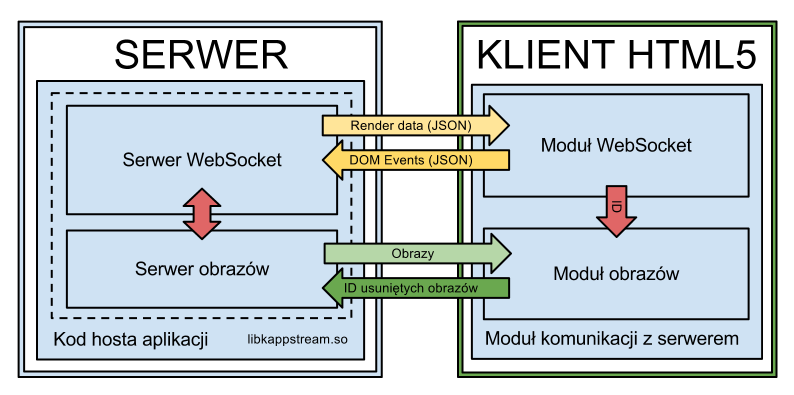
\includegraphics[width=1.0\linewidth]{img/arch-socket}
\caption{Schemat komunikacji z modułem WebSocket.}
\label{fig:arch-socket}
\end{figure}

\begin{figure}[H]
\centering
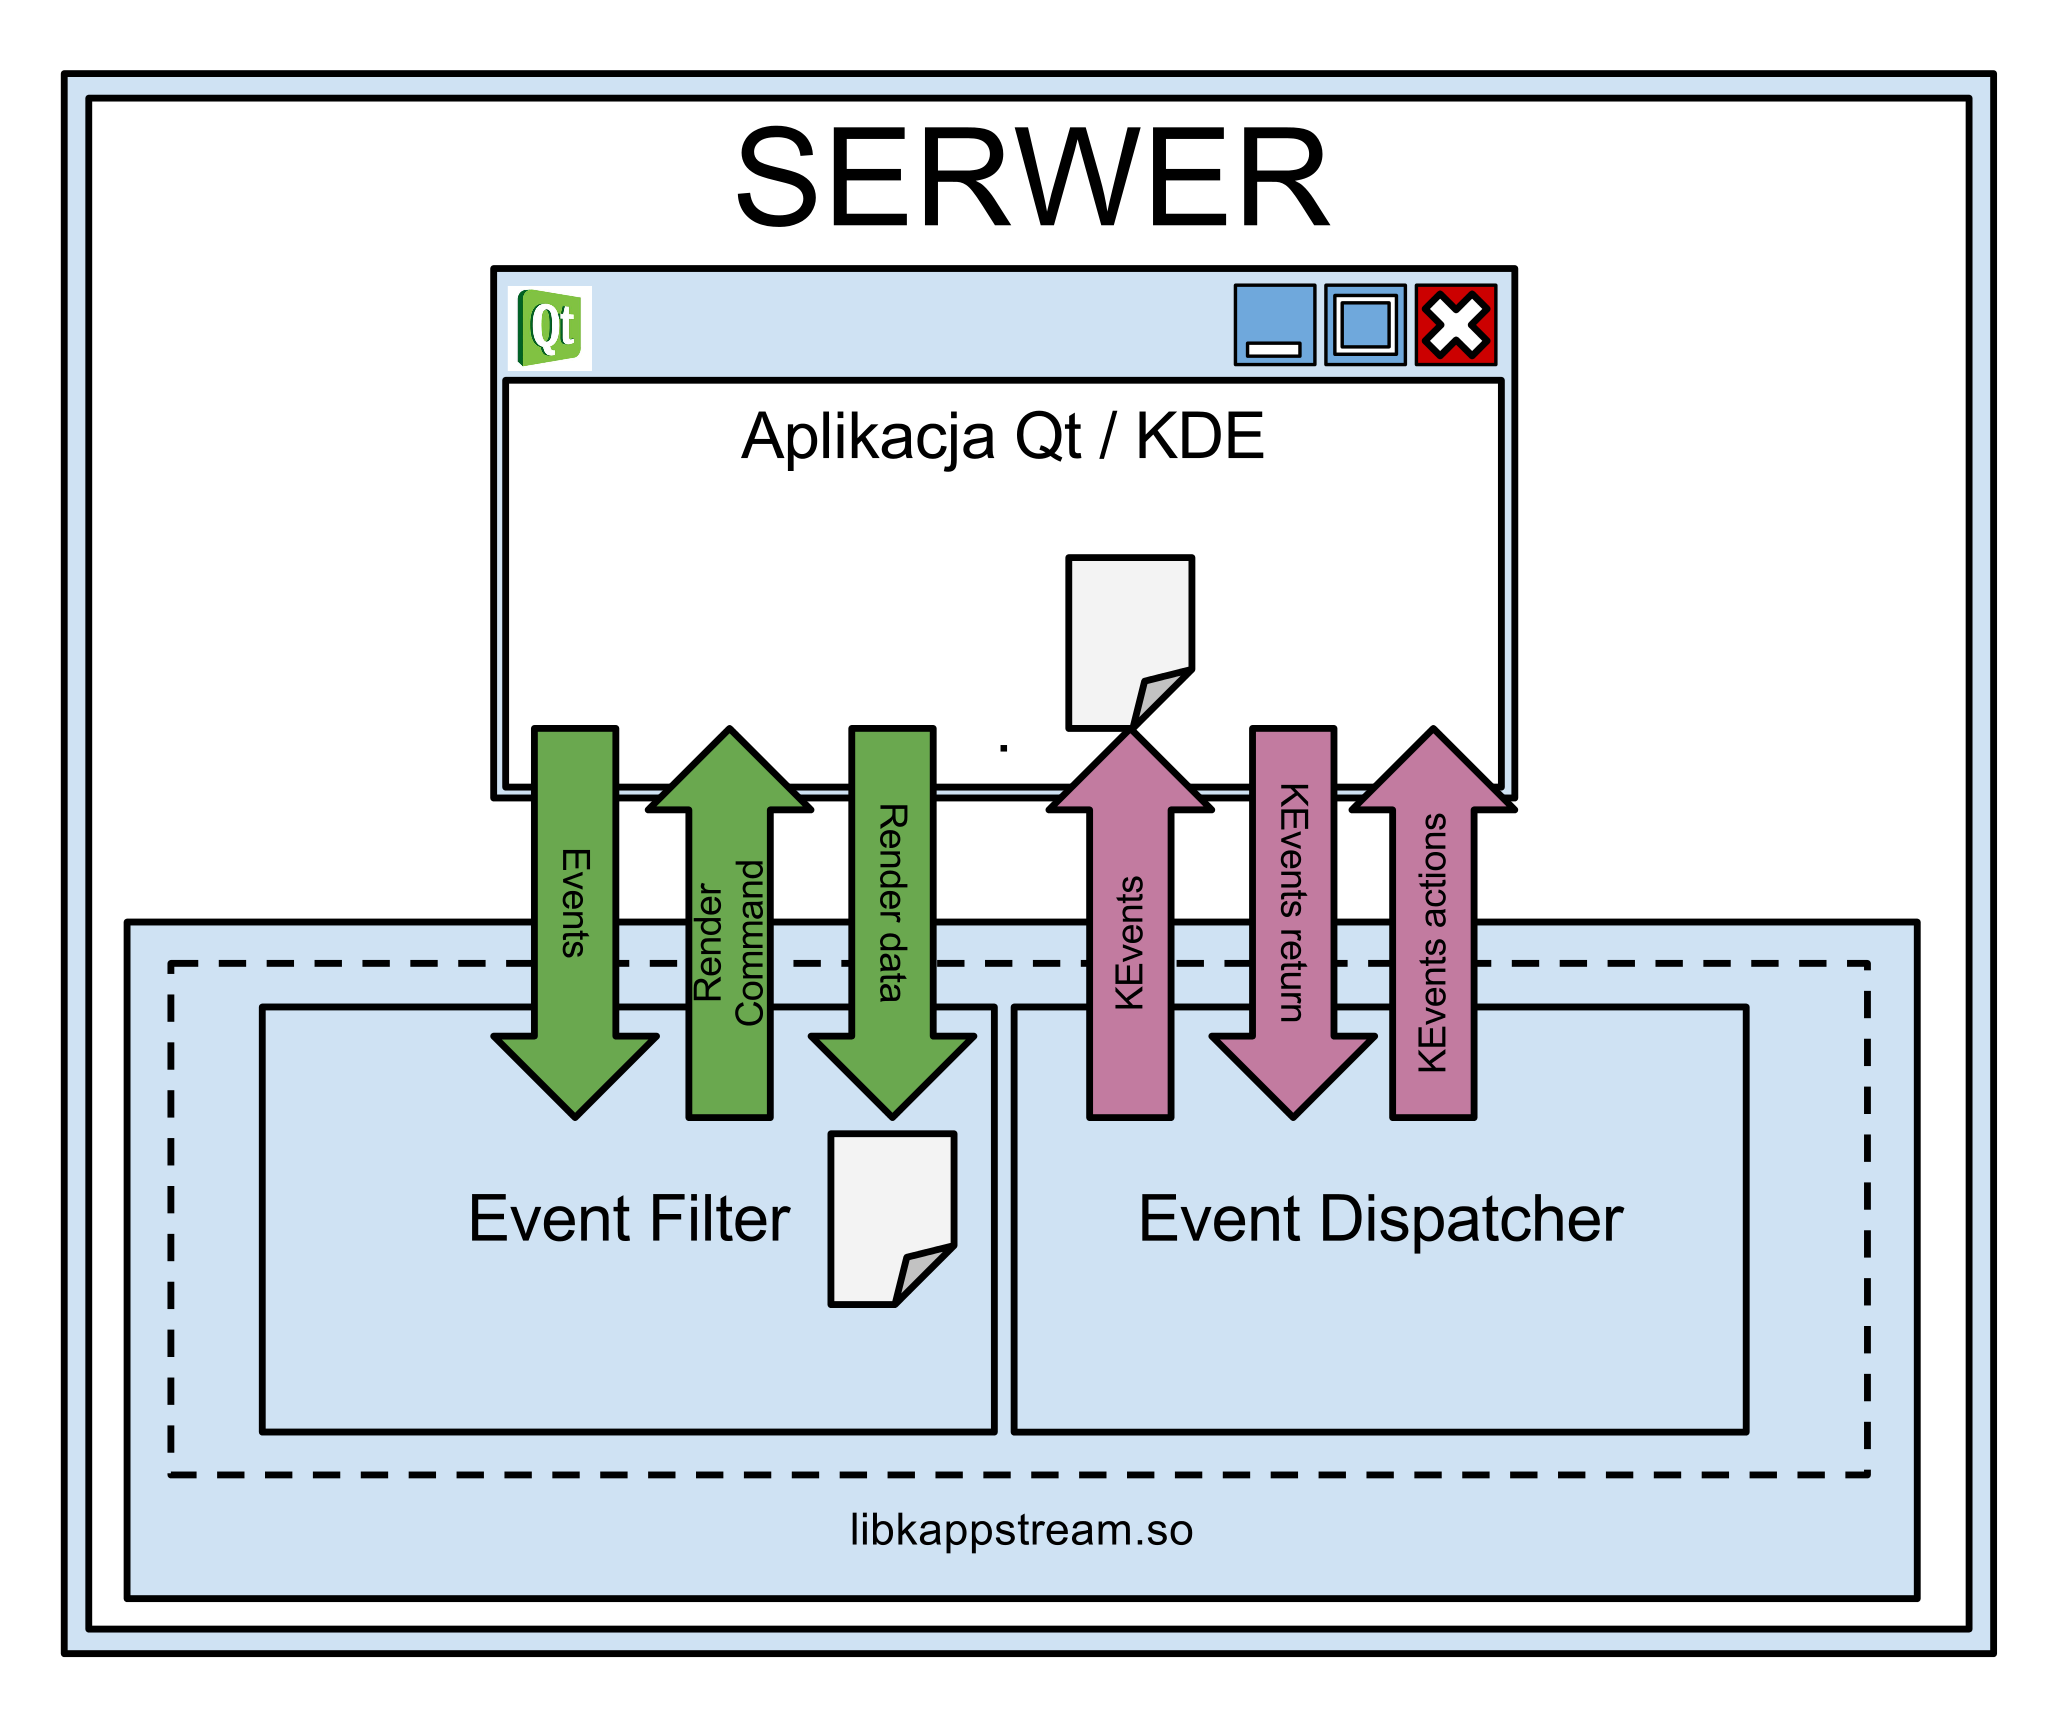
\includegraphics[width=1.0\linewidth]{img/arch-hook}
\caption{Schemat powiązań modułu WebSocket z aplikacją \emph{Qt/KDE}.}
\label{fig:arch-hook}
\end{figure}